%!TEX encoding = IsoLatin

%% Document is article 
\documentclass[a4paper]{article}

%% ----------------------------------------------------- PACKAGES ----------------------------------------------------- %%
\usepackage{coolArticle}

%% ---------------------------------------------------- DOCUMENT ---------------------------------------------------- %%
\begin{document}

\noindent \textsc{Gallos-Montbrun} Gr�goire\\
\textsc{Faury} Louis 
	\titlebox{0.6}{Model Predictive Control}{Exercise \#5 - \textcolor{blue}{Group 2}}
	
	\vspace{10pt}
	\paragraph{} We consider the following system : 
	\begin{equation}\label{eq::system}
		\begin{aligned}
			x^+ &= Ax + Bu \\
			y_k &= Cx +d
		\end{aligned}
	\end{equation}
	where : 
	\begin{equation}
		A = \begin{pmatrix} 0.7115 & -0.4345 \\ 0.4345 & 0.8853\end{pmatrix}, \qquad B = \begin{pmatrix} 0.2173 \\ 0.0573 \end{pmatrix}, \qquad C = \begin{pmatrix} 1 & 0 \end{pmatrix}
	\end{equation}
	We suppose that the disturbance $d$, as well as the initial state $x_0$ are unknown, and consider the following input constraints : 
	\begin{equation}
		-3 \leq u \leq 3
	\end{equation}
	
	\section{Exercise 1}
	{
		\paragraph{} Let us define $\hat{x}_k$ to be the current state of an estimator of the state $x$, with dynamic : 
		\begin{equation}
			\hat{x}_{k+1} = A\hat{x}_k + Bu_k + L(C\hat{x}_k + \hat{d}_k-y_k) 
		\end{equation}
		were $\hat{d}_k$ is the current estimate of the unknown disturbance. \\
		\paragraph{} Therefore the error $e_k = \begin{pmatrix} x_k - \hat{x}_k \\ d -\hat{d}_{k+1}\end{pmatrix}$  of the augmented state follows the dynamics : 
		\begin{equation}
			e_{k+1} = \left[\begin{pmatrix} A & 0 \\ 0 & I \end{pmatrix} + L\begin{pmatrix} C & 1\end{pmatrix}\right]e_k
		\end{equation}
		Since $(A,C)$ is full-rank, and since $\begin{pmatrix} A - I & 0 \\ C  & 1\end{pmatrix}$ has full column-rank, it exists $L$ so that $\begin{pmatrix} A & 0 \\ 0 & I \end{pmatrix} + L\begin{pmatrix} C & 1\end{pmatrix}$ is Hurwitz. 
		
		\begin{figure}[h!]
			\begin{minipage}{0.5\linewidth}
				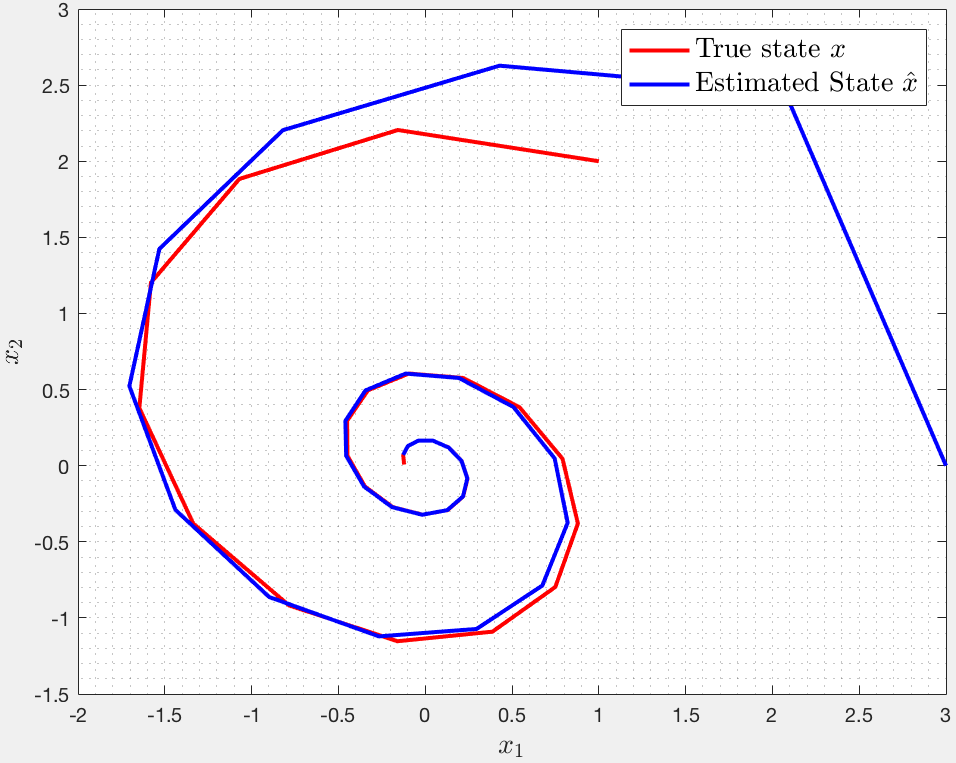
\includegraphics[width=\linewidth]{xest}
				\caption{State dynamics and estimation}
				\label{fig::xest}
			\end{minipage}
			\begin{minipage}{0.5\linewidth}
				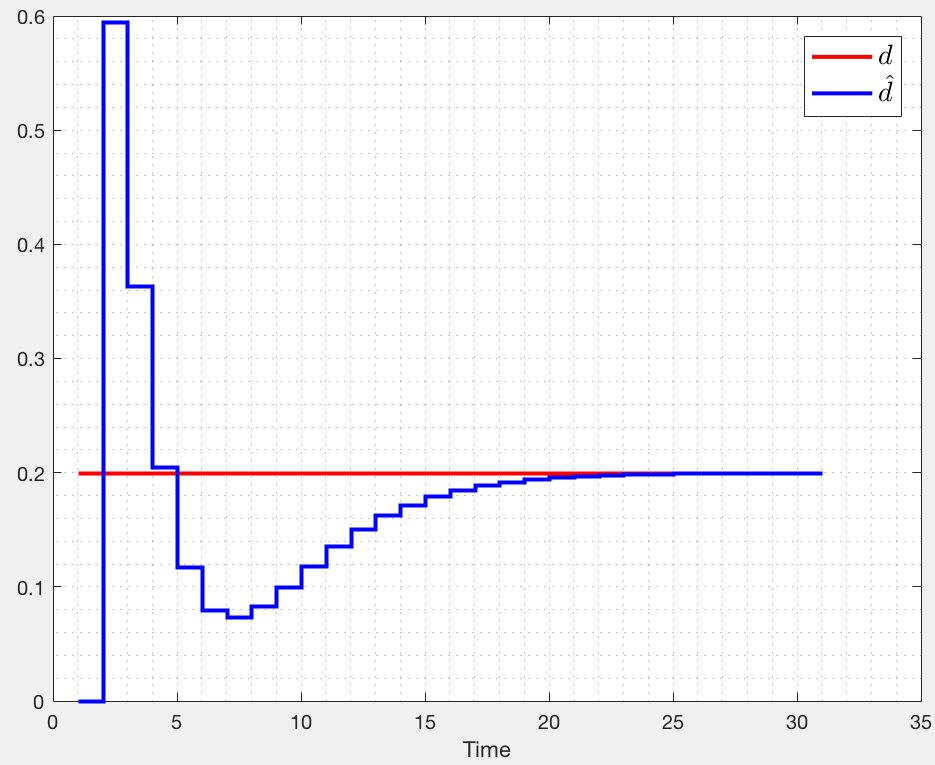
\includegraphics[width=0.95\linewidth]{dest}
				\caption{Disturbance estimation}
				\label{fig::dest}
			\end{minipage}
		\end{figure}
		
		\paragraph{} With such $L$, the error is steered to $0$ and we get \textbf{unbiased asymptotic estimators} for $x$ and $d$. With the Matlab command \texttt{place}, we can determine $L$ so that the resulting dynamics have given eigenvalues. Figures (\ref{fig::xest}) and (\ref{fig::dest}) show the convergence of $\hat{x}_k$ and $\hat{d}_k$ to their true values, with $u=0$ (the uncontrolled system is stable). In this example, we took the poles to be : 
		\begin{equation}
			\lambda_1 = 0.5, \quad \lambda_2 = 0.6, \quad \lambda_3 = 0.7
		\end{equation}
		
	}
    
    \section{Exercise 2}
	{
		\paragraph{} 
        In this exercise, we consider that at instant $k$ we dispose from an estimate $\hat{x}_k$ for the current state as well as an estimate $\hat{d}_k$ for the disturbance. We intend to compute $u_s$, the steady state input that minimizes $u^2$ while allowing the output $y$ to follow the reference $r$ and respecting input constraints.
        
        \paragraph{}
        At steady state, equation (\ref{eq::system}) writes:
        \begin{equation}
		\begin{aligned}
			x_s &= Ax_s + Bu_s \\
			r &= Cx_s +d
		\end{aligned}
		\end{equation}
        which is equivalent to:
        \begin{equation}
		\begin{bmatrix}
			I-A & -B\\
			C & 0
        \end{bmatrix}
        \begin{bmatrix}
			x_s\\
			u_s
        \end{bmatrix}
        =	\begin{bmatrix}
			0\\
			r-C_d d
        \end{bmatrix}
		\end{equation}
        
        \paragraph{}
        However, actual disturbance $d$ is unknown, we therefore use $\hat{d}_k$ to approach it with the following minimization problem:
        
        \begin{equation}
        		\begin{aligned}
				&\quad \quad \quad \quad \quad \quad \quad \min_{u_s, x_s} u_s^2\\
				&\text{ s.t }  \left\{
					\begin{aligned}
						& \begin{bmatrix} I-A & -B\\ C & 0 \end{bmatrix} \begin{bmatrix} x_s\\ u_s\end{bmatrix} =	\begin{bmatrix} 0\\ r-C_d \hat{d}_k\end{bmatrix}\\
                       	& -3 \leq u_s \leq 3
					\end{aligned}\right.
			\end{aligned}
        \end{equation}
        
      \paragraph{}
      We solve this minimization problem using YALMIP quadratic programming methods on Matlab.	
	}
    
     \section{Exercise 3}
	{
		\paragraph{}
        In this exercise we design an MPC controller for reference tracking for the disturbed system. We use stage costs $Q=I$ and $R=1$ The terminal set is easy to compute: since there is no constraint on the state of the system, and since the system is stable, $\chi_f = \mathbb{R}^2$ is a convenient terminal set. Corresponding terminal cost is: 
        \begin{equation}
        V_f(x_N) = (x_N - x_s)^TP((x_N - x_s)), \textrm{ with } P - A^TPA = Q.
        \end{equation}
        
        \paragraph{}
        the resulting minimization problem solved at each time step is therefore:
        \begin{equation}
        \begin{aligned}
			&\min_{\Delta u_i, \Delta x_i} \sum_{i=0}^{N-1} \Delta x_i^TQ \Delta x_i + \Delta u_i^TR \Delta u_i + \Delta x_N^TP \Delta x_N\\
				& \text{ s.t }  \left\{
					\begin{aligned}
                    	& \Delta x_0 = \Delta \hat{x}\\
                        & \forall i \in\{0,\hdots, N-1\} \Delta x_{i+1} = A\Delta x_i + B \Delta u_i \\
						&\forall i \in\{0,\hdots, N-1\}, \, -3+u_s \leq \Delta u_i \leq 3+u_s\\
						& \Delta x_N \in \mathbb{R}^2         
					\end{aligned}\right.
		\end{aligned}
        \end{equation}
        
        where $\Delta x_i = (x_i - x_s)$, and $\Delta u_i = (u_i - u_s)$ with $u_s$ and $x_s$ computed at each time step according to exercise 2.
        
        \paragraph{}
        Figures (\ref{fig::xtraj_0.5}), (\ref{fig::u_0.5}) and (\ref{fig::y_0.5}) display the result of the closed loop MPC simulation with $r=0.5$ and $N=5$ as horizon. We clearly see that output $y$ converges to the reference and that control $u$ always satisfy the constraints. Moreover, as in exercise 1, state estimate converges to the actual state.
        \begin{figure}[h!]
        		\begin{minipage}{0.33\linewidth}
			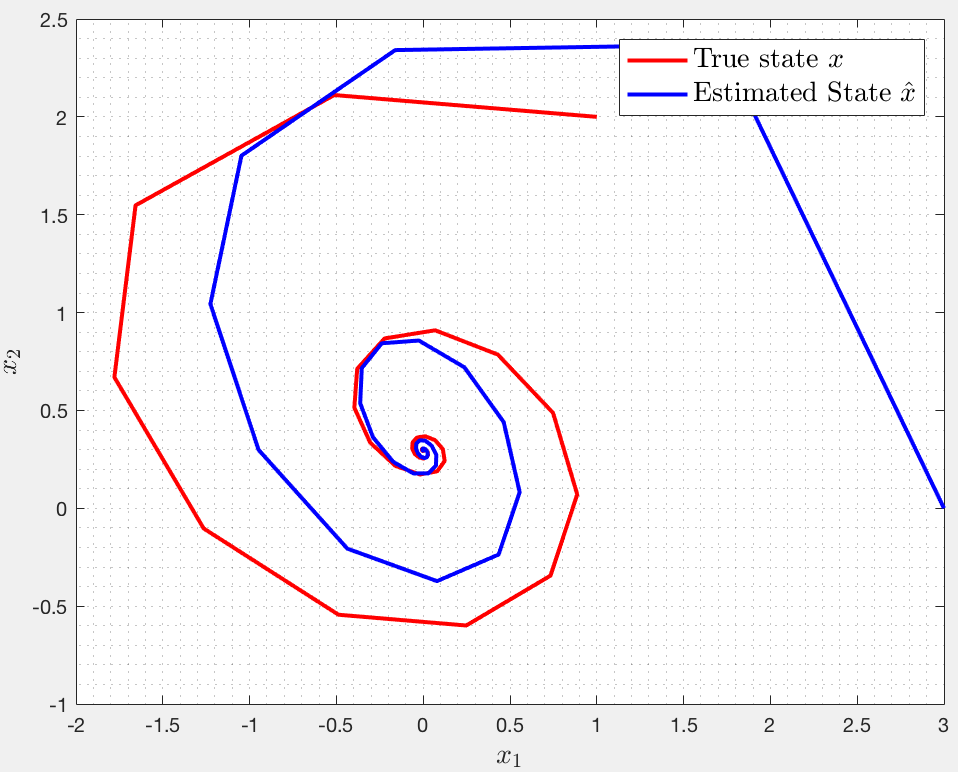
\includegraphics[width=\linewidth]{xtraj_05}
			\caption{Trajectory estimation, $r=0.5$}
			\label{fig::xtraj_0.5}
		\end{minipage}
		\begin{minipage}{0.33\linewidth}
			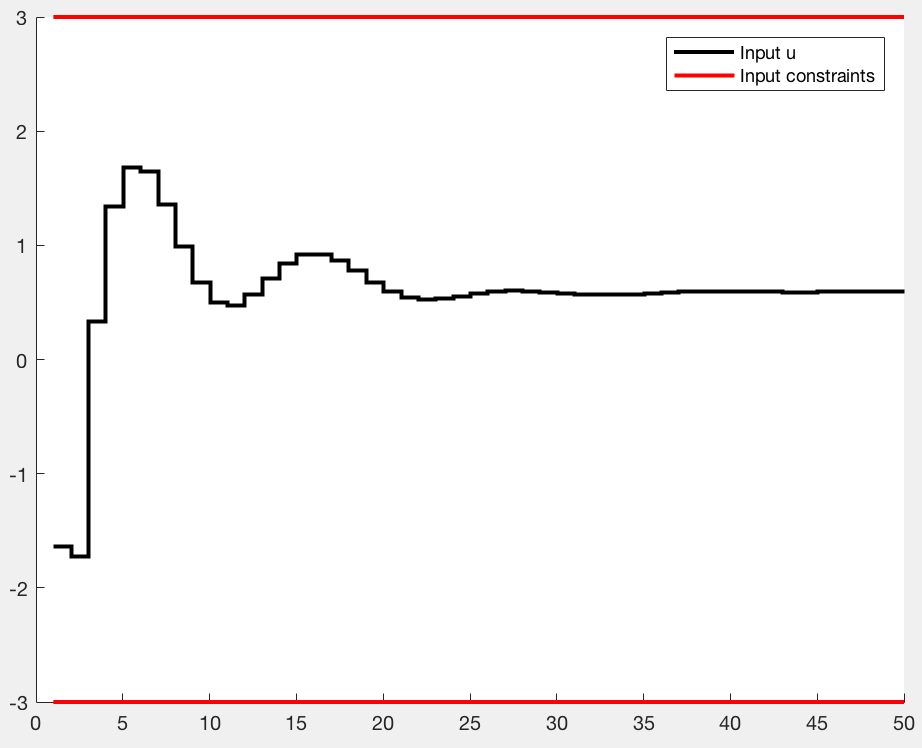
\includegraphics[width=\linewidth]{u_05}
			\caption{Inputs, $r=0.5$}
			\label{fig::u_0.5}
		\end{minipage}
		\begin{minipage}{0.33\linewidth}
			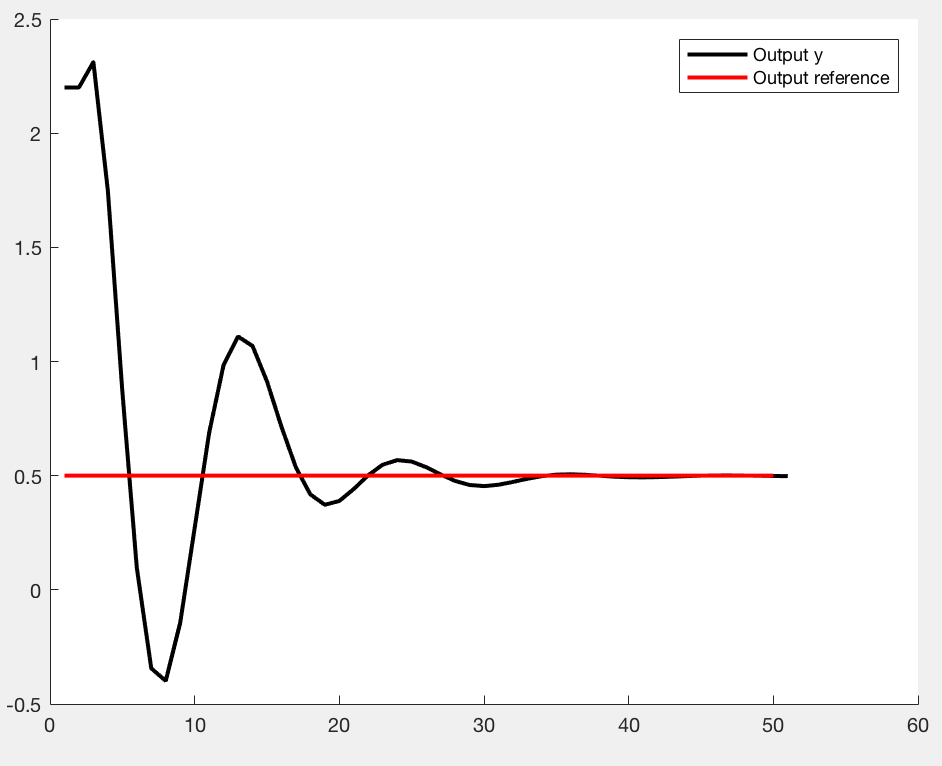
\includegraphics[width=\linewidth]{y_05}
			\caption{Output estimation, $r=0.5$}
			\label{fig::y_0.5}
		\end{minipage}
        \end{figure}
        
        \paragraph{}
         Figures (\ref{fig::xtraj_1}), (\ref{fig::u_1}) and (\ref{fig::y_1}) show similar result with $r=1$.
         
          \begin{figure}[h!]
        		\begin{minipage}{0.33\linewidth}
			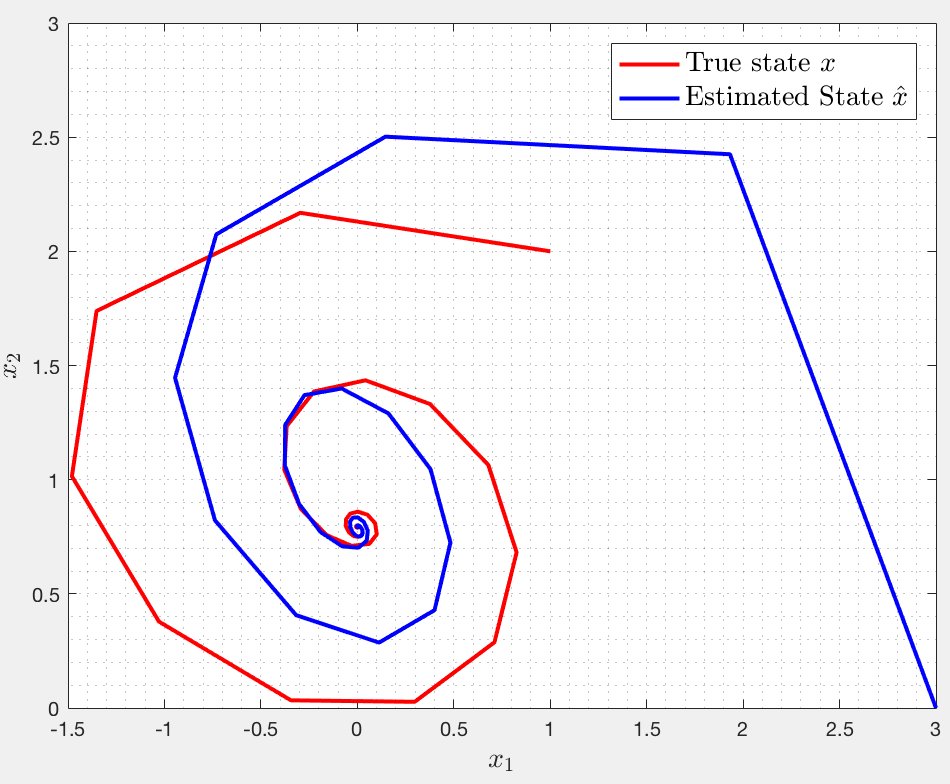
\includegraphics[width=\linewidth]{xtraj_1}
			\caption{Trajectory estimation, $r=1$}
			\label{fig::xtraj_1}
		\end{minipage}
		\begin{minipage}{0.33\linewidth}
			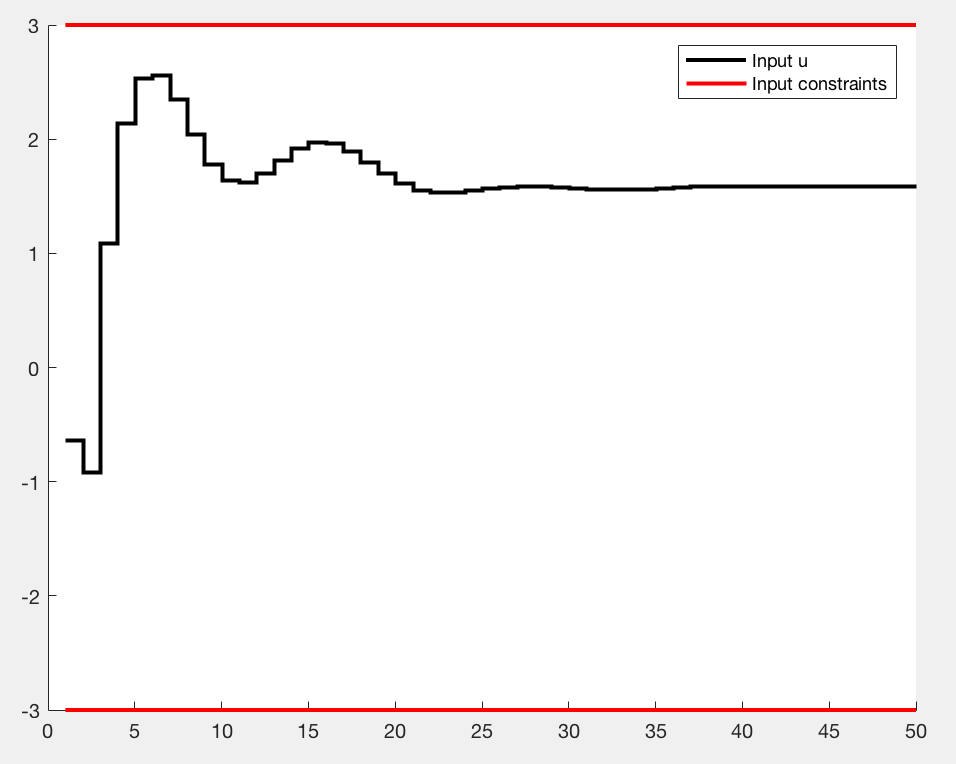
\includegraphics[width=\linewidth]{u_1}
			\caption{Inputs, $r=1$}
			\label{fig::u_1}
		\end{minipage}
		\begin{minipage}{0.33\linewidth}
			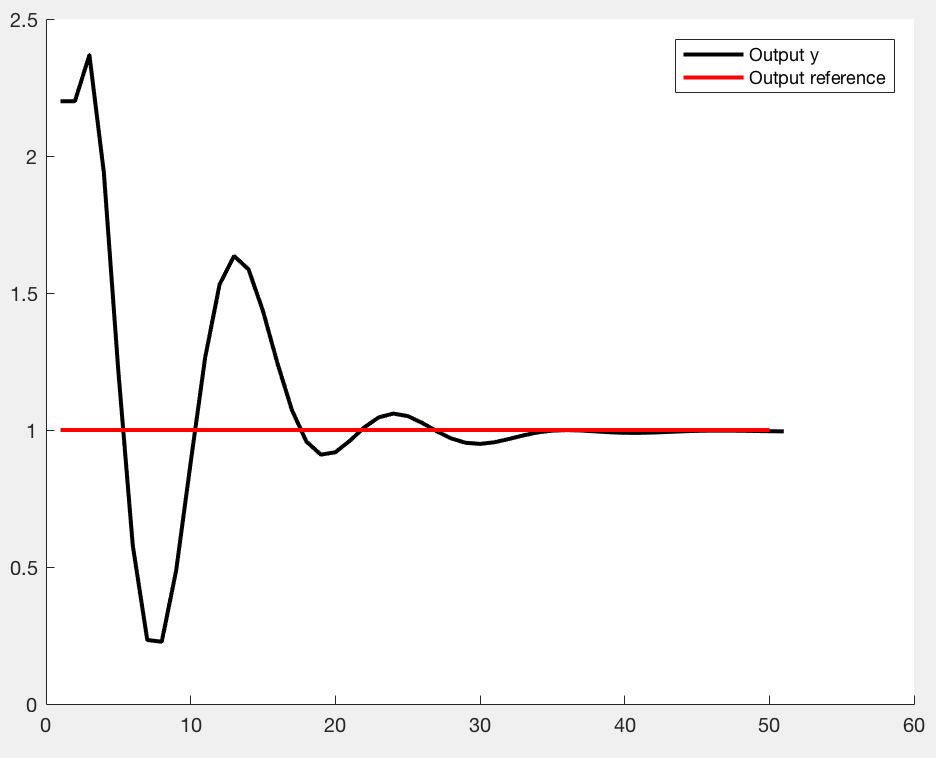
\includegraphics[width=\linewidth]{y_1}
			\caption{Output estimation, $r=1$}
			\label{fig::y_1}
		\end{minipage}
        \end{figure}
        
	}
   
   
\end{document}